\subsection{迭代器模式(Iterator)}

\subsubsection{迭代器模式简介}

迭代器模式提供一种方法来顺序访问聚合对象中的一系列数据,而不暴露聚合对象的内部表示。

\subsubsection{迭代器模式在项目中的应用}

\begin{figure}[h]
  \centering
  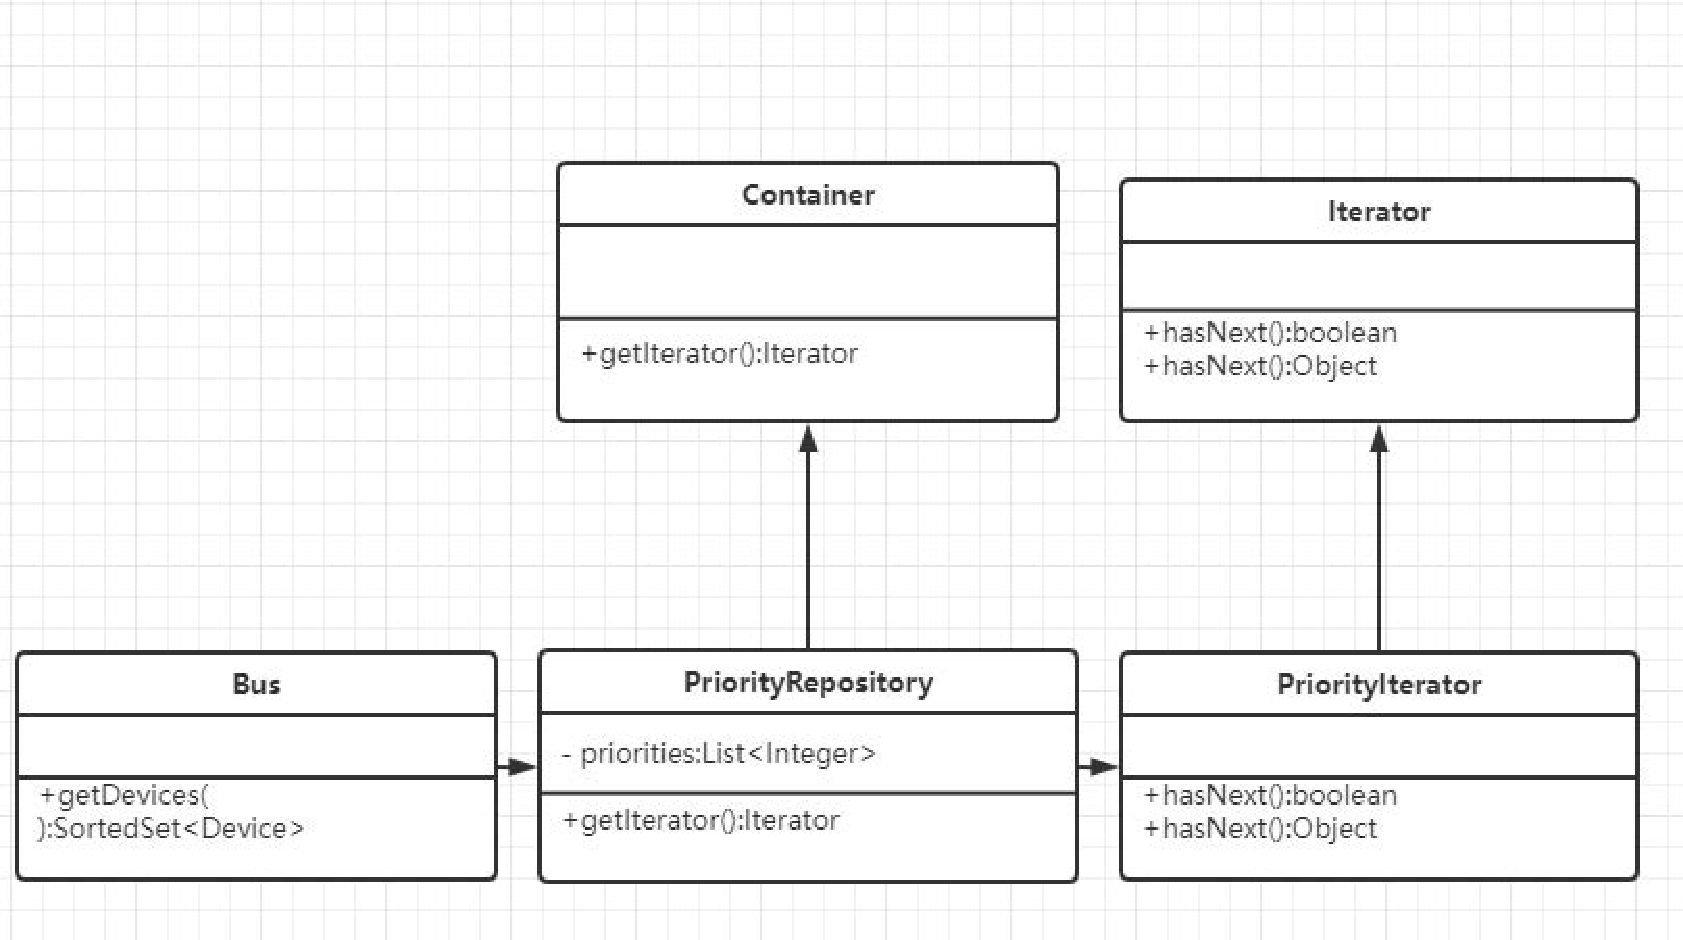
\includegraphics[width=0.9\textwidth]{figures/迭代器模式.pdf}
  \caption{迭代器模式在 Slow6502 中的类图}
\end{figure}

使用迭代器可以更方便地遍历容器中的数据。在模拟器中,容器通常包含大量的数据,并且这些数据可能非常复杂。如果想要对这些数据进行遍历,就必须手动编写代码来完成这一过程。这样做不仅耗时,而且容易出错。使用迭代器可以简化遍历容器中的数据的过程。迭代器可以把复杂的遍历过程封装在一个对象中,只需要调用该对象的相关方法就可以完成遍历。这样做可以让您更快速地完成遍历,避免出现错误。此外,使用迭代器还可以让代码更容易理解和维护。迭代器可以把复杂的遍历过程分解成一系列简单的步骤,使代码更加清晰易懂。这样,程序员可以更容易地查看和修改代码,避免出现错误。

总的来说,使用迭代器可以更方便地遍历容器中的数据,并让代码更容易理解和维护。
